\section{Diseño del Sistema de Control}

    \subsection{Control en Cascada} % LIC -> FIC

La arquitectura de control base seleccionada para cada línea de los depósitos corresponde a un esquema en Cascada. Esta topología se justifica teóricamente por la existencia de dos dinámicas temporales claramente separadas: la dinámica rápida del actuador y la tubería (flujo), y la dinámica lenta de acumulación de masa (nivel del estanque).

El esquema se compone de dos lazos anidados:
\begin{itemize}
    \item \textbf{Lazo Interno (Esclavo - FIC):} Su objetivo es controlar el caudal inyectado al sistema. Posee una dinámica rápida y su función principal es rechazar las perturbaciones locales del actuador (como variaciones en la presión de la línea, desgaste mecánico de la bomba o histéresis) antes de que afecten a la variable principal. Al sintonizar este lazo, el conjunto actuador-tubería se linealiza desde la perspectiva del controlador maestro.
    \item \textbf{Lazo Externo (Maestro - LIC):} Su objetivo es controlar el nivel del estanque ($h_i$). Su salida de control no ataca directamente al variador de frecuencia, sino que establece el *Setpoint* dinámico ($SP_{flujo}$) que el lazo esclavo debe seguir.
\end{itemize}

Matemáticamente, la señal de control final $u(t)$ enviada al variador de frecuencia es calculada por el algoritmo discreto del FIC, cuyo error se define como $e_{flujo}[k] = LIC_{out}[k] - FIT[k]$. Esta separación de dinámicas permite utilizar sintonías más agresivas en el control de nivel sin comprometer la estabilidad ante imperfecciones mecánicas.
    \subsection{Lógica de Selección (Override)} % Bloques TY
    Como el sistema es sub-actuado ya que cuenta con 4 salidas pero sólo 2 actuadores, no es posible controlar los estanque $1$ y $4$ o $2$ y $3$.

    Es por esto que se implementa un algoritmo de selección entre las señales al actuador, esto se desglosa en la siguiente tabla:

    $$\begin{bmatrix}
    >: \text{Flujo mayor}\\
    <: \text{Flujo menor}\\
  e: \text{Mayor error}
    \end{bmatrix}$$
\clearpage
    \subsection{Feed-Forward (Prealimentación)} % G_h y G_w


El control retroalimentado (Feedback) tradicional posee una limitación inherente: requiere que exista un error en la variable de proceso para poder actuar. Para compensar esta inercia, se implementa una arquitectura de prealimentación o \textit{Feedforward} (FF), la cual mide las variables de entrada al sistema e inyecta una acción de control antes de que la variable controlada se vea afectada.

\begin{figure}[ht]
  \begin{center}
    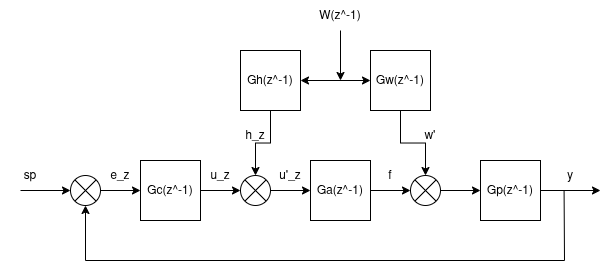
\includegraphics[width=0.95\textwidth]{img/ff.png}
  \end{center}
  \caption{}\label{fig:ff}
\end{figure}
\subsubsection{Obtención Matemática: Compensación de Perturbaciones}

Considérese un sistema donde la salida $y(z^{-1})$ se ve afectada tanto por la acción de control $u_z$ a través de la planta $G_p(z^{-1})$ y el actuador $G_a(z^{-1})$, como por una perturbación medible $W(z^{-1})$ a través de su propia dinámica $G_w(z^{-1})$. La ecuación en el dominio $Z$ es:
\[
  Y(z^{-1}) =G_p(z^{-1}) \left[ (u_{z}(z^{-1}) + h_{h}(z^{-1})) G_a(z^{-1}) + W(z^{-1}) G_w(z^{-1}) \right]
\]
\[
Y(z^{-1}) = G_p(z^{-1})\left[ (u_{z}(z^{-1}) + W(z^{-1})G_h(z^{-1})) G_a(z^{-1})  + W(z^{-1}) G_w(z^{-1})\right]
\]
\[ 
  Y(z^{-1}) = G_p(z^{-1})\left[u_z(z^{-1})G_a(z^{-1})G_p(z^{-1}) + W(z^{-1})G_h(z^{-1})G_a(z^{-1}) + W(z^{-1})G_w(z^{-1})\right]  
\]

\begin{equation}
  Y(z^{-1}) = \underbrace{(Sp - Pv)G_c(z^{-1})G_a(z^{-1})G_p(z^{-1})}_{\text{PID}} + \underbrace{W(z^{-1})G_h(z^{-1})G_a(z^{-1})G_p(z^{-1}) + W(z^{-1})G_w(z^{-1})G_p(z^{-1})}_{\text{Feed-Forward}}  
  \label{eq:ff2}
\end{equation}

\clearpage


El objetivo del compensador de perturbaciones es lograr una invariancia perfecta, es decir, que el efecto de $W(z^{-1})$ sobre $Y(z^{-1})$ sea nulo ($Y(z^{-1}) = 0$ asumiendo $u_{z}=0$). Igualando a cero la contribución de la perturbación, se despeja la acción de control anticipatoria:
\[
  0 = W(z^{-1})G_h(z^{-1})G_a(z^{-1})G_p(z^{-1}) + W(z^{-1})G_w(z^{-1})G_p(z^{-1}) 
\]

\begin{equation}
  G_h(z^{-1}) = -\frac{G_w(z^{-1})}{G_a(z^{-1})} 
  \label{eq:G_w}
\end{equation}
Definiendo el bloque compensador como $
  G_h(z^{-1}) = -\frac{G_w(z^{-1})}{G_a(z^{-1})} 
$, se logra la cancelación algebraica de la perturbación entrante.

\subsubsection{Obtención Matemática: Seguimiento de Referencia (Setpoint)}
Se puede aplicar un raciocinio idéntico para mejorar el seguimiento de la referencia ($SP$). En lugar de esperar a que el integrador del PID acumule la energía necesaria para alcanzar el nivel deseado, se puede pre-calcular el esfuerzo de control exacto. 

Es fundamental destacar que \textbf{no se invierte la dinámica completa de la planta} (lo cual requeriría la derivada de la referencia y generaría un esfuerzo de control irrealizable). En su lugar, el Feedforward de Setpoint invierte únicamente la \textbf{ganancia estática} del proceso. 

En sistemas con dinámicas complejas como el de los 4 estanques, esta ganancia estática contiene la principal no linealidad del sistema (la fuga parabólica de Torricelli). Al inyectar una señal de prealimentación que es la inversa exacta de esta no linealidad ($G_{sp} = G_{estatico}^{-1}$), se logran dos objetivos simultáneos:

\begin{enumerate}
    \item Proporcionar al actuador la energía base requerida para sostener el nivel del Setpoint deseado en estado estacionario.
    \item Linealizar el sistema desde la perspectiva del lazo cerrado, permitiendo que el controlador PID solo deba encargarse de corregir las inercias transitorias dinámicas y los pequeños errores de modelación.
\end{enumerate}


\begin{figure}[ht]
  \begin{center}
    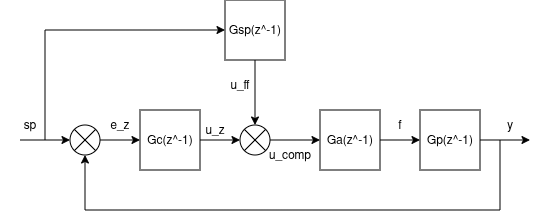
\includegraphics[width=0.8\textwidth]{img/ff_sp.png}
  \end{center}
  \caption{}\label{fig:ffsp}
\end{figure}

Ignorando la perturbación y la acción del controlador temporalmente, se busca que la salida alcance la referencia ($Y(z^{-1}) = SP(z^{-1})$) utilizando exclusivamente una acción precalculada $U_{FF\_SP}(z^{-1})$:

\begin{align}
    SP(z^{-1}) &= U_{FF\_SP}(z^{-1}) G_a(z^{-1}) G_p(z^{-1}) \\
    U_{FF\_SP}(z^{-1}) &= SP(z^{-1}) \frac{1}{G_a(z^{-1}) G_p(z^{-1})}
\end{align}

Definiendo este segundo bloque como $G_{sp}(z^{-1}) = \frac{1}{G_a(z^{-1}) G_p(z^{-1})}$, se establece un control de \textit{2 Grados de Libertad}, donde el Feedforward proporciona el esfuerzo base y el PID se encarga únicamente de corregir errores dinámicos y no linealidades residuales no modeladas.

\subsubsection{Aplicación a las Ecuaciones de Diferencias de la Planta}
Para aplicar esta teoría lineal a los estanques no lineales, evaluamos la derivada del balance de masas en estado estacionario ($\frac{dh}{dt} = 0$). Tomando como ejemplo el Estanque 1 (que sufre la perturbación de caudal del Estanque 3), la Ecuación \ref{eq:edo_h1} se iguala a cero.

Forzando que en estado estacionario el nivel alcance el Setpoint ($h_1 = SP_1$), y despejando la acción de control de la bomba ($u_1$), obtenemos la ley de control Feedforward pura (sin considerar aún la acción del PID):
\begin{align}
    0 &= -a_1 \sqrt{2g \cdot SP_1} + a_3 \sqrt{2g \cdot h_3} + \gamma_1 k_1 u_1 \nonumber \\
    \gamma_1 k_1 u_1 &= a_1 \sqrt{2g \cdot SP_1} - a_3 \sqrt{2g \cdot h_3} \nonumber \\
    u_1 &= \underbrace{\frac{a_1 \sqrt{2g \cdot SP_1}}{\gamma_1 k_1}}_{\text{Término } G_h \text{ (Referencia)}} - \underbrace{\frac{a_3 \sqrt{2g \cdot h_3}}{\gamma_1 k_1}}_{\text{Término } C_w \text{ (Perturbación)}}
\end{align}

Al integrar esto con el algoritmo digital dentro del PLC, la señal de control total en el instante discreto $[k]$ resulta en la suma de prealimentación y el control retroalimentado:
\begin{equation}
    u_{total}[k] = u_{PID}[k] + \frac{a_1 \sqrt{2g \cdot SP_1[k]}}{\gamma_1 k_1} - \frac{a_3 \sqrt{2g \cdot h_3[k]}}{\gamma_1 k_1}
\end{equation}

\clearpage
\subsection{Arquitecturas de Inyección del Feedforward en Cascada}

Al implementar la estrategia de prealimentación junto con un control en cascada (LIC $\rightarrow$ FIC) en Texto Estructurado, existen dos topologías matemáticas válidas para inyectar el Feedforward. La elección depende de si se prioriza la robustez del lazo o la velocidad de rechazo de la perturbación.

\subsubsection{Arquitectura 1: Inyección en el Setpoint del Lazo Esclavo}
En este enfoque, el Feedforward se suma a la salida del controlador maestro (LIC). Dado que el Setpoint del lazo de flujo (FIC) debe estar en unidades de caudal ($cm^3/s$ o $L/min$), la ecuación de prealimentación \textbf{no debe incluir la ganancia de la bomba ($k_1$)}. 

La secuencia de cálculo discreto en el instante $[k]$ es:
\begin{align}
    Q_{FF}[k] &= \frac{a_1 \sqrt{2g \cdot SP_1[k]}}{\gamma_1} - \frac{a_3 \sqrt{2g \cdot h_3[k]}}{\gamma_1} \label{eq:ff_caudal} \\
    SP_{FIC}[k] &= CV_{LIC}[k] + Q_{FF}[k] \label{eq:sp_fic_sum} \\
    u_1[k] &= CV_{FIC}[k] \label{eq:u_arch1}
\end{align}

\textbf{Ventaja:} Es la arquitectura más robusta. El FIC es el único encargado de gobernar la señal hacia el actuador ($u_1[k]$), por lo que su término integral mantiene el control total sobre la linealidad de la bomba sin sufrir problemas de \textit{windup} por señales externas.

\subsubsection{Arquitectura 2: Inyección a la Salida del Lazo Esclavo}
En este enfoque, el controlador de nivel (LIC) ataca directamente al Setpoint del flujo, y el Feedforward se inyecta en la etapa final, sumándose a la salida del FIC. En este caso, el Feedforward debe calcular \textbf{esfuerzo de control (Hz o Voltaje)}, por lo que la ganancia de la bomba ($k_1$) es indispensable en el denominador.

La secuencia de cálculo discreto en el instante $[k]$ es:
\begin{align}
    SP_{FIC}[k] &= CV_{LIC}[k] \label{eq:sp_fic_direct} \\
    u_{FF}[k] &= \frac{a_1 \sqrt{2g \cdot SP_1[k]}}{\gamma_1 k_1} - \frac{a_3 \sqrt{2g \cdot h_3[k]}}{\gamma_1 k_1} \label{eq:ff_esfuerzo} \\
    u_1[k] &= CV_{FIC}[k] + u_{FF}[k] \label{eq:u_arch2}
\end{align}

\textbf{Ventaja y Precaución:} Esta arquitectura garantiza un rechazo de perturbaciones casi instantáneo, ya que la señal de compensación ($u_{FF}[k]$) llega directamente al actuador saltándose la inercia dinámica del algoritmo del FIC. Sin embargo, al sumar una señal externa a la salida de un PID discreto implementado en Texto Estructurado, es estrictamente necesario aplicar técnicas de recálculo hacia atrás (\textit{back-calculation}) en el término integral del FIC; de lo contrario, el controlador asumirá que la perturbación fue un error propio e intentará cancelarla, desestabilizando el sistema.



\subsubsection{Solución Híbrida: Doble Inyección (Feedforward Coordinado)}

Si los requerimientos del proceso exigen la velocidad de reacción de la \textbf{Arquitectura 2} (inyección directa al actuador), pero se desea evitar el conflicto con la acción Proporcional e Integral del lazo esclavo en un entorno de Texto Estructurado puro, la solución matemática es implementar una \textit{Doble Inyección}.

Este método consiste en calcular simultáneamente el Feedforward en unidades de caudal ($Q_{FF}$) y en unidades de esfuerzo de control ($u_{FF}$), inyectándolos en ambos extremos del controlador esclavo (FIC) al mismo tiempo. De esta forma, se logra la corrección instantánea en la bomba, mientras se enmascara la perturbación modificando el Setpoint del FIC, lo que mantiene el error del esclavo cercano a cero y anula cualquier intento de contramedida.

La secuencia de cálculo discreto para la doble inyección en el instante $[k]$ es:

1. \textbf{Cálculo del requerimiento físico (Caudal):}
   $$Q_{FF}[k] = \frac{a_1 \sqrt{2g \cdot SP_1[k]}}{\gamma_1} - \frac{a_3 \sqrt{2g \cdot h_3[k]}}{\gamma_1}$$

 2. \textbf{Transformación a esfuerzo de control:}
   $$u_{FF}[k] = \frac{Q_{FF}[k]}{k_1}$$

 3. \textbf{Inyección 1: Ajuste del Setpoint (Pre-compensación):}
   $$SP_{FIC}[k] = CV_{LIC}[k] + Q_{FF}[k]$$

 4. \textbf{Cálculo del error y algoritmo del controlador (FIC):}
   $$e_{FIC}[k] = SP_{FIC}[k] - FIT_1[k]$$
   $$CV_{FIC}[k] = \text{PID}(e_{FIC}[k])$$

   5. \textbf{Inyección 2: Acción directa al actuador (Salida final):}
   $$u_1[k] = CV_{FIC}[k] + u_{FF}[k]$$

---

\textbf{Análisis de Dinámica:} Al momento de ocurrir la perturbación, $u_{FF}[k]$ altera el variador de frecuencia en el mismo ciclo de \textit{Scan}, garantizando un rechazo inmediato. Físicamente, el flujo $FIT_1$ cambia drásticamente. Sin embargo, como el término $Q_{FF}[k]$ fue sumado al $SP_{FIC}$, la ecuación del error ($e_{FIC}$) evalúa esta alza de flujo como el seguimiento exitoso de su nueva referencia. El lazo esclavo se mantiene estable y la cascada no se rompe..


\subsection{Selección de Arquitectura Feedforward en Cascada}

La elección entre inyectar la prealimentación en el Setpoint del esclavo (Arquitectura 1), en la salida del esclavo (Arquitectura 2) o utilizar una Doble Inyección (Arquitectura 3), no posee una respuesta única. El ingeniero de control debe evaluar los siguientes criterios de diseño:

\begin{enumerate}
    \item \textbf{Dinámica Relativa (Velocidad de Respuesta):}
    \begin{itemize}
        \item Si la dinámica del lazo esclavo (FIC) es al menos 5 a 10 veces más rápida que la perturbación, la \textbf{Arquitectura 1 (Setpoint)} es suficiente. El FIC reaccionará tan rápido al cambio de su referencia que el error temporal será despreciable.
        \item Si el actuador es lento o posee un tiempo muerto significativo, se prefiere la \textbf{Doble Inyección} para enviar el comando de voltaje inmediatamente y ganar tiempo físico, mientras se coordina con el PID.
    \end{itemize}

    \item \textbf{Nivel de Ruido en la Perturbación (Chattering):}
    \begin{itemize}
        \item El cálculo del Feedforward depende directamente de las mediciones de los sensores (en este caso, los transmisores de nivel $LIT$). Si esta señal es ruidosa (ej. oleaje en el estanque), la inyección directa a la salida transmitirá ese ruido amplificado directamente a la bomba, causando desgaste mecánico prematuro.
        \item En presencia de ruido, la \textbf{Arquitectura 1} es superior, ya que el algoritmo integral del FIC actúa como un filtro pasabajos (amortiguador) natural antes de que la señal llegue a la bomba.
    \end{itemize}

    \item \textbf{Herramientas de Programación (Bloques vs. ST puro):}
    \begin{itemize}
        \item Si el autómata dispone de bloques de control avanzados (como la instrucción \texttt{PIDE} en ControlLogix) que gestionan automáticamente el \textit{back-calculation} en su pin \texttt{FF}, la \textbf{Doble Inyección} se vuelve trivial de implementar y es altamente recomendada.
        \item Si el control debe ser programado desde cero mediante ecuaciones en diferencias en Texto Estructurado (ST), la \textbf{Arquitectura 1} es mandatoria para evitar un desarrollo de software excesivamente complejo y propenso a fallos matemáticos por \textit{Integral Windup}.
    \end{itemize}

    \item \textbf{Saturación y Seguridad del Actuador:}
    \begin{itemize}
        \item En la inyección a la salida, si el PID pide 40 Hz y el FF pide 20 Hz, la suma exige 60 Hz. Como el variador satura a 50 Hz, el sistema físico se limita, pero el PID interno no lo sabe y su integrador colapsa. Al inyectar en el Setpoint (Arquitectura 1), el FIC gestiona la saturación internamente y congela su integrador (\textit{Anti-Windup}) de forma natural.
    \end{itemize}
\end{enumerate}
